\documentclass[a4paper, 12pt]{article}
\usepackage[utf8]{inputenc}
\usepackage[ngerman]{babel}
\usepackage{graphicx}
\usepackage{abstract}
\usepackage{amssymb}
\usepackage{color}
\usepackage{hyperref}
\usepackage{amsmath}
\usepackage{multicol}
\usepackage{amssymb}
\usepackage[onehalfspacing]{setspace}
\usepackage[left=2.5cm, right=2.5cm, top=2.5cm, bottom=2.5cm]{geometry}
\usepackage{listings}
\setlength{\parindent}{0ex}
\begin{document}
\begin{multicols}{2}

\includegraphics[width=0.3\textwidth]{bilder/Uni-Bremen_Logo.png}
\\
\end{multicols}
\begin{center}
{\LARGE\bfseries MaMBA Projekt: LoRa Kommunikation}
\\
{\Large Aufbau der Kommunikationsstruktur\\unter der Verwendung von LoRa}
\end{center}
\begin{figure}[h!]
\centering
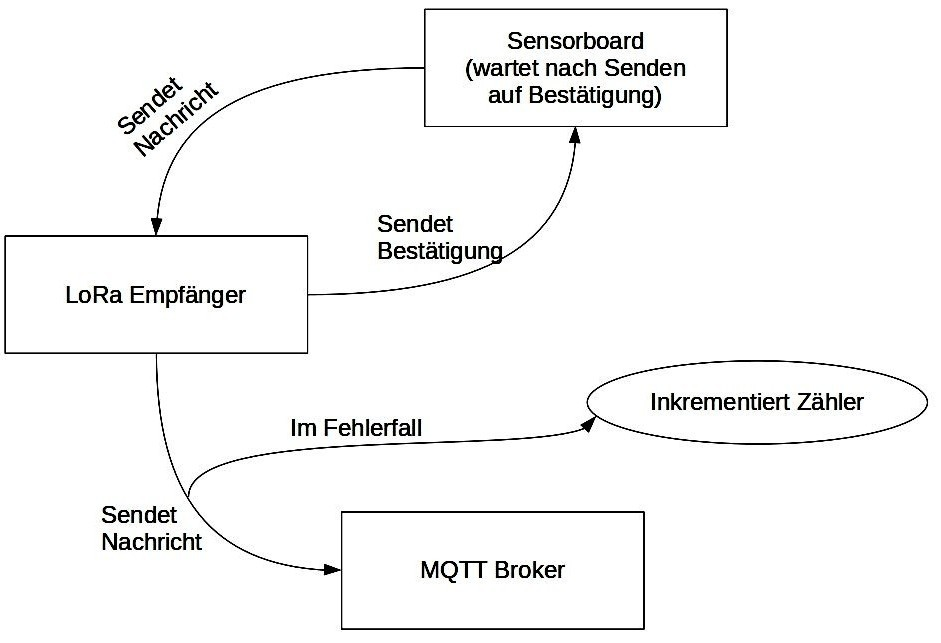
\includegraphics[width=1\textwidth]{bilder/expl.jpg}
\caption{Allgemeiner Ablauf, vereinfacht}\label{abb:ablauf}
\end{figure}
Im Folgenden soll diskutiert werden, wie der Kommunikationsweg von der Erfassung der Messdaten bis zu ihrer Darstellung abläuft. Beginnend auf dem Sensorboard werden hier circa alle zwei Sekunden Messwerte aller angeschlossenen Sensoren aufgenommen. Dann werden alle dreißig Sekunden die zu diesem Zeitpunkt aktuellen Messwerte in eine interne Datenstruktur des Sensorboards gespeichert. Im Anschluss wird der neuste Wert aus der Datenstruktur an den LoRa Empfänger gesendet. Wenn dieses Senden erfolgreich war, werden die gesendeten Messwerte aus der Datenstruktur gelöscht. Die Struktur der Nachricht ist folgende:
\begin{table}[h!]
\centering
\begin{tabular}{|c|c|c|c|}
\hline
Messwerte 	&	8 Bit (Sensorstatus 0/1)	&	8 Bit (Paket-ID)	&	1 Bit\\ 
\hline
\end{tabular}
\end{table}\\
Dabei enthält die gesendete Nachricht an erster Stelle die Messwerte, danach eine acht Bit (so viele Sensoren sind auf dem Sensorboard angebracht) große Zahl, wobei jede null für einen funktionierenden und jede eins für einen nicht funktionierenden beziehungsweise angeschlossenen Sensor zählt. Darauf folgend wird dann eine individuelle Paket-ID vergeben, welche ebenfalls klarstellt, von welchem Sensorboard die Nachricht stammt und anhand derer sich mit einer vorangegangenen oder folgenden Paket-ID ermitteln lässt, ob eine Nachricht verloren gegangen ist. Als letzter Teil einer Nachricht steht dann noch eine ein Bit große Zahl. Bei dieser bedeutet eine null, dass normale Werte an der ersten Stelle stehen, eine eins signalisiert, dass die Werte außerhalb definierter Grenzen liegen.\\ 

Der Abstand der Nachrichten von dem Sensorboard an den LoRa Empfänger beträgt dreißig Sekunden, da eine hohe Datendichte (die entsteht wenn beispielsweise nach jeder Messung eine Nachricht gesendet wird) im Normalbetrieb nicht von Nöten ist, da die Messwerte sich ohnehin nicht in relevanten Größenordnungen ändern. Außerdem ist der Abstand zwischen der Änderung der Messwerte auf der Anzeige und in der Datenbank so konstant. Wenn eine Änderung der gemessenen Werte außerhalb definierter Grenzen liegt, so wird die Messung nach dem erläuterten Schema sofort versendet. Zu dem sendet das Sensorboard alle zwei Sekunden ein Heartbeatsignal an den LoRa Empfänger. Wenn drei aufeinanderfolgende Heartbeatsignale ausfallen, so wird eine Warnung in abgesetzt, welche bedeutet, dass das betreffende Sensorboard eine Inspektion benötigt. So ist auch gewährleistet, dass ein eventuelles Ausfallen eines Sensorboards schneller als in dreißig Sekunden erkannt wird.\\

Insgesamt vier Sensorboards werden installiert, davon jeweils zwei im Ober- und Untergeschoss. In jeder Etage verhalten sich die beiden Sensorboards gleich zu einander: Ein Sensorboard verhält sich wie oben beschrieben. Das andere Sensorboard sendet nicht alle dreißig Sekunden, sondern alle zwei Minuten eine Nachricht und wird im Folgenden als Backupboard bezeichnet. Die Messwerte der Nachricht der Sensorboards, welche alle dreißig Sekunden Nachrichten senden werden immer verglichen. Wenn diese Differenz größer als ein zuvor festgelegter Wert ist oder das bereits erwähnte Heartbeatsignal nicht die genannte Bedingung erfüllt, so wird das Zeitintervall der Backupboards von zwei Minuten auf dreißig Sekunden gesetzt und eine Warnung abgesetzt (s.o.). Wenn dann nach der Inspektion festgestellt wird, dass die Abweichung im Rahmen war, wird eine Eingabe auf dem Tablet getätigt und das Backupboard geht wieder in den vorigen Betriebszustand zurück.\\

Sobald bei dem LoRa Empfänger eine Nachricht angekommen ist, so wird eine Bestätigung an das Sensorboard zurück gesendet. Danach wird die aktuelle Paket-ID mit der vorigen Paket-ID verglichen. Wenn diese nicht aufeinander folgende Zahlen sind, so wurde ein Paket verloren. Dieser Fall ist allerdings äußerst unwahrscheinlich, da das Sensorboard nach dem Versenden jeder Nachricht auf eine Bestätigung seitens des LoRa Empfängers wartet. Wenn diese Bestätigung nicht nach einem festgelegten Zeitraum empfangen wird, so wird die Nachricht erneut versendet. Wenn dieser Vorgang dreimal wiederholt wurde, wird die Nachricht verworfen (also aus der internen Datenstruktur des Sensorboards gelöscht). Die bei dem LoRa Empfänger angekommene Nachricht wird dann versucht an den MQTT Broker zu senden. Wenn das nicht gelingt, wird ein interner Zähler inkrementiert. Danach wird versucht die nächste Nachricht zu senden. Wenn dies gelingt, so wird ebenfalls der Zähler (wenn er nicht null ist) veröffentlicht um die Anzahl der verlorenen Werte anzuzeigen und anschließend wieder auf den Wert null gesetzt, ansonsten wird der Zähler wieder inkrementiert. Diese Funktionalität kann später geändert werden, was ansonsten den aktuellen Zeitplan sprengt. Angekommen bei dem MQTT Broker werden die Daten mit Openhab (Tablet) dargestellt und mit einem Zeitstempel in die Datenbank gespeichert. Im Anschluss werden die Daten ausgelesen und mit Hilfe von Grafana dargestellt.
\end{document}